

%\documentclass[a4paper]{jarticle}


\section{mbonsai 系列データによる決定木生成\label{sect:mbonsai}}
\index{mbonsai@mbonsai}
本コマンドは、系列パターンを説明変数として利用可能な決定木モデル構築コマンドである。
系列データの解析は様々な応用分野において適用できる。
顧客が購入したブランドの順序,スーパーや百貨店における売り場の巡回パターン,
傷病の発症順序,これらは全て系列データとして解析できる。
本コマンドのオリジナルのアイデアは、九州大学の研究チームによって開発されたBONSAI\cite{SSS94}にあり、
分子生物学におけるアミノ酸配列を解析することを目的に構築された手法である。
この手法をビジネスデータに応用する中で、いくつかの改良を加えたものが本コマンドで、
以下のような特徴をもつ。

\begin{itemize}
 \item カテゴリ系列データから有用なパターンを抽出し、その有無を決定木における節点の条件とすることができる。
 \item モデル精度を高めるように、系列を構成するアイテムをグルーピングすることができる。
 \item 複数の系列データを扱うことができる。
 \item 系列データ以外にも数値変数、カテゴリ変数も含めてモデル化ができる。
 \item 決定木モデルの構築モードと未知データを与えての予測モードがある。
 \item 3つ以上のクラス分類問題にも対応している。
\end{itemize}

まず直感的理解を得るために,以下に例を示す。
ある小売店における顧客別のブランド\verb|a,b,c|の購入系列と、
その店からの離反の有無についてのデータが表\ref{tbl:mbonsai_inp1}に示されている。
ブランドの購入順序が顧客の離反に関係しているとの仮説のもと、
離反の有無を目的変数に、そしてブランドの購買順序に関する部分的なパターン(ここでのパターンとは部分文字列、例えば
、"ab","cbb"を考えればよい。パターンの定義の詳細は次節を参照のこと。)を説明変数にして決定木モデルを構築する。
このような説明変数としてのパターンは候補パターンと呼ばれ、モデルの精度に寄与するであろうパターンが事前に生成され(その方法も次節を参照のこと)、
それらのパターンを0-1変数としてデータセットが作成される(表\ref{tbl:mbonsai_inp2})。
このデータセットから一般的な方法で決定木が構築される。
実際に本コマンドを用いて作成された決定木が図\ref{fig:mbonsai_bonsai1}に示されている。

\begin{table}[htbp]
\begin{center}
\begin{tabular}{ll}

\begin{minipage}{0.5\hsize}
\begin{center}
\caption{系列データの例。
一行が一人の顧客に対応し、目的変数として、それぞれの顧客が離反したかどうかが示されている。
「ブランド系列」項目に示されたアルファベットa,b,cは、顧客が購入したブランドを表しており、
それぞれに示された順序で購入したことを意味する。
\label{tbl:mbonsai_inp1}}
{\small
\begin{tabular}{lc}
\hline
ブランド系列&離反 \\
\hline
bcaba   & yes \\
bcabcaa & yes \\
aaabac  & yes \\
caa     & yes \\
cca     & no  \\
cacbc   & no  \\
bcc     & no  \\
acca    & no  \\
\hline
\end{tabular} 
}
\end{center}
\end{minipage}

\begin{minipage}{0.5\hsize}
\begin{center}
\caption{
表\ref{tbl:mbonsai_inp1}のブランド系列項目から抜き出された部分的な購入パターンを説明変数とし(候補パターンと呼ぶ)、
全サンプルに対してパターンを含むかどうかの0-1データに変換されたデータセットの例。
一行目の顧客は部分パターン"a","b","c","ab"を含んでいるが、"aa","cc"は含んでいない。
\label{tbl:mbonsai_inp2}}
{\small
\begin{tabular}{cccccccl}
\hline
a&b&c&aa&ab&cc&$\cdots$&離反 \\
\hline
1&1&1&0&1&0&& yes \\
1&1&1&1&1&0&& yes \\
1&1&1&1&1&0&& yes \\
1&0&1&1&0&0&$\cdots$& yes \\
1&0&1&0&0&1&& no \\
1&1&1&0&0&0&& no \\
0&1&1&0&0&1&& no \\
1&0&1&0&0&1&& no \\
\hline
\end{tabular} 
}
\end{center}
\end{minipage}

\end{tabular} 
\end{center}
\end{table} 


\begin{table}[htbp]
\begin{center}
\begin{tabular}{ll}

\begin{minipage}{0.5\hsize}
\begin{center}
%\begin{figure}[htpb]
\centering
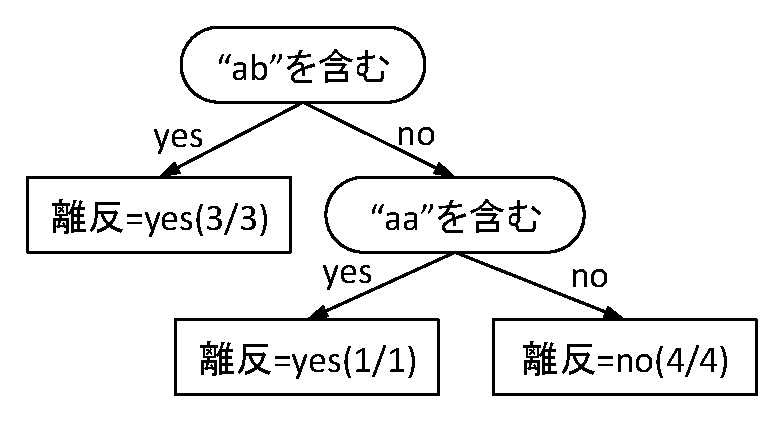
\includegraphics[scale=0.5,clip]{./figure/bonsai1.eps}
\caption{BONSAIによる離反顧客モデルの構築例}
\label{fig:mbonsai_bonsai1}
%\end{figure}
\end{center}
\end{minipage}

\begin{minipage}{0.5\hsize}
\begin{center}
%\begin{figure}[htpb]
\centering
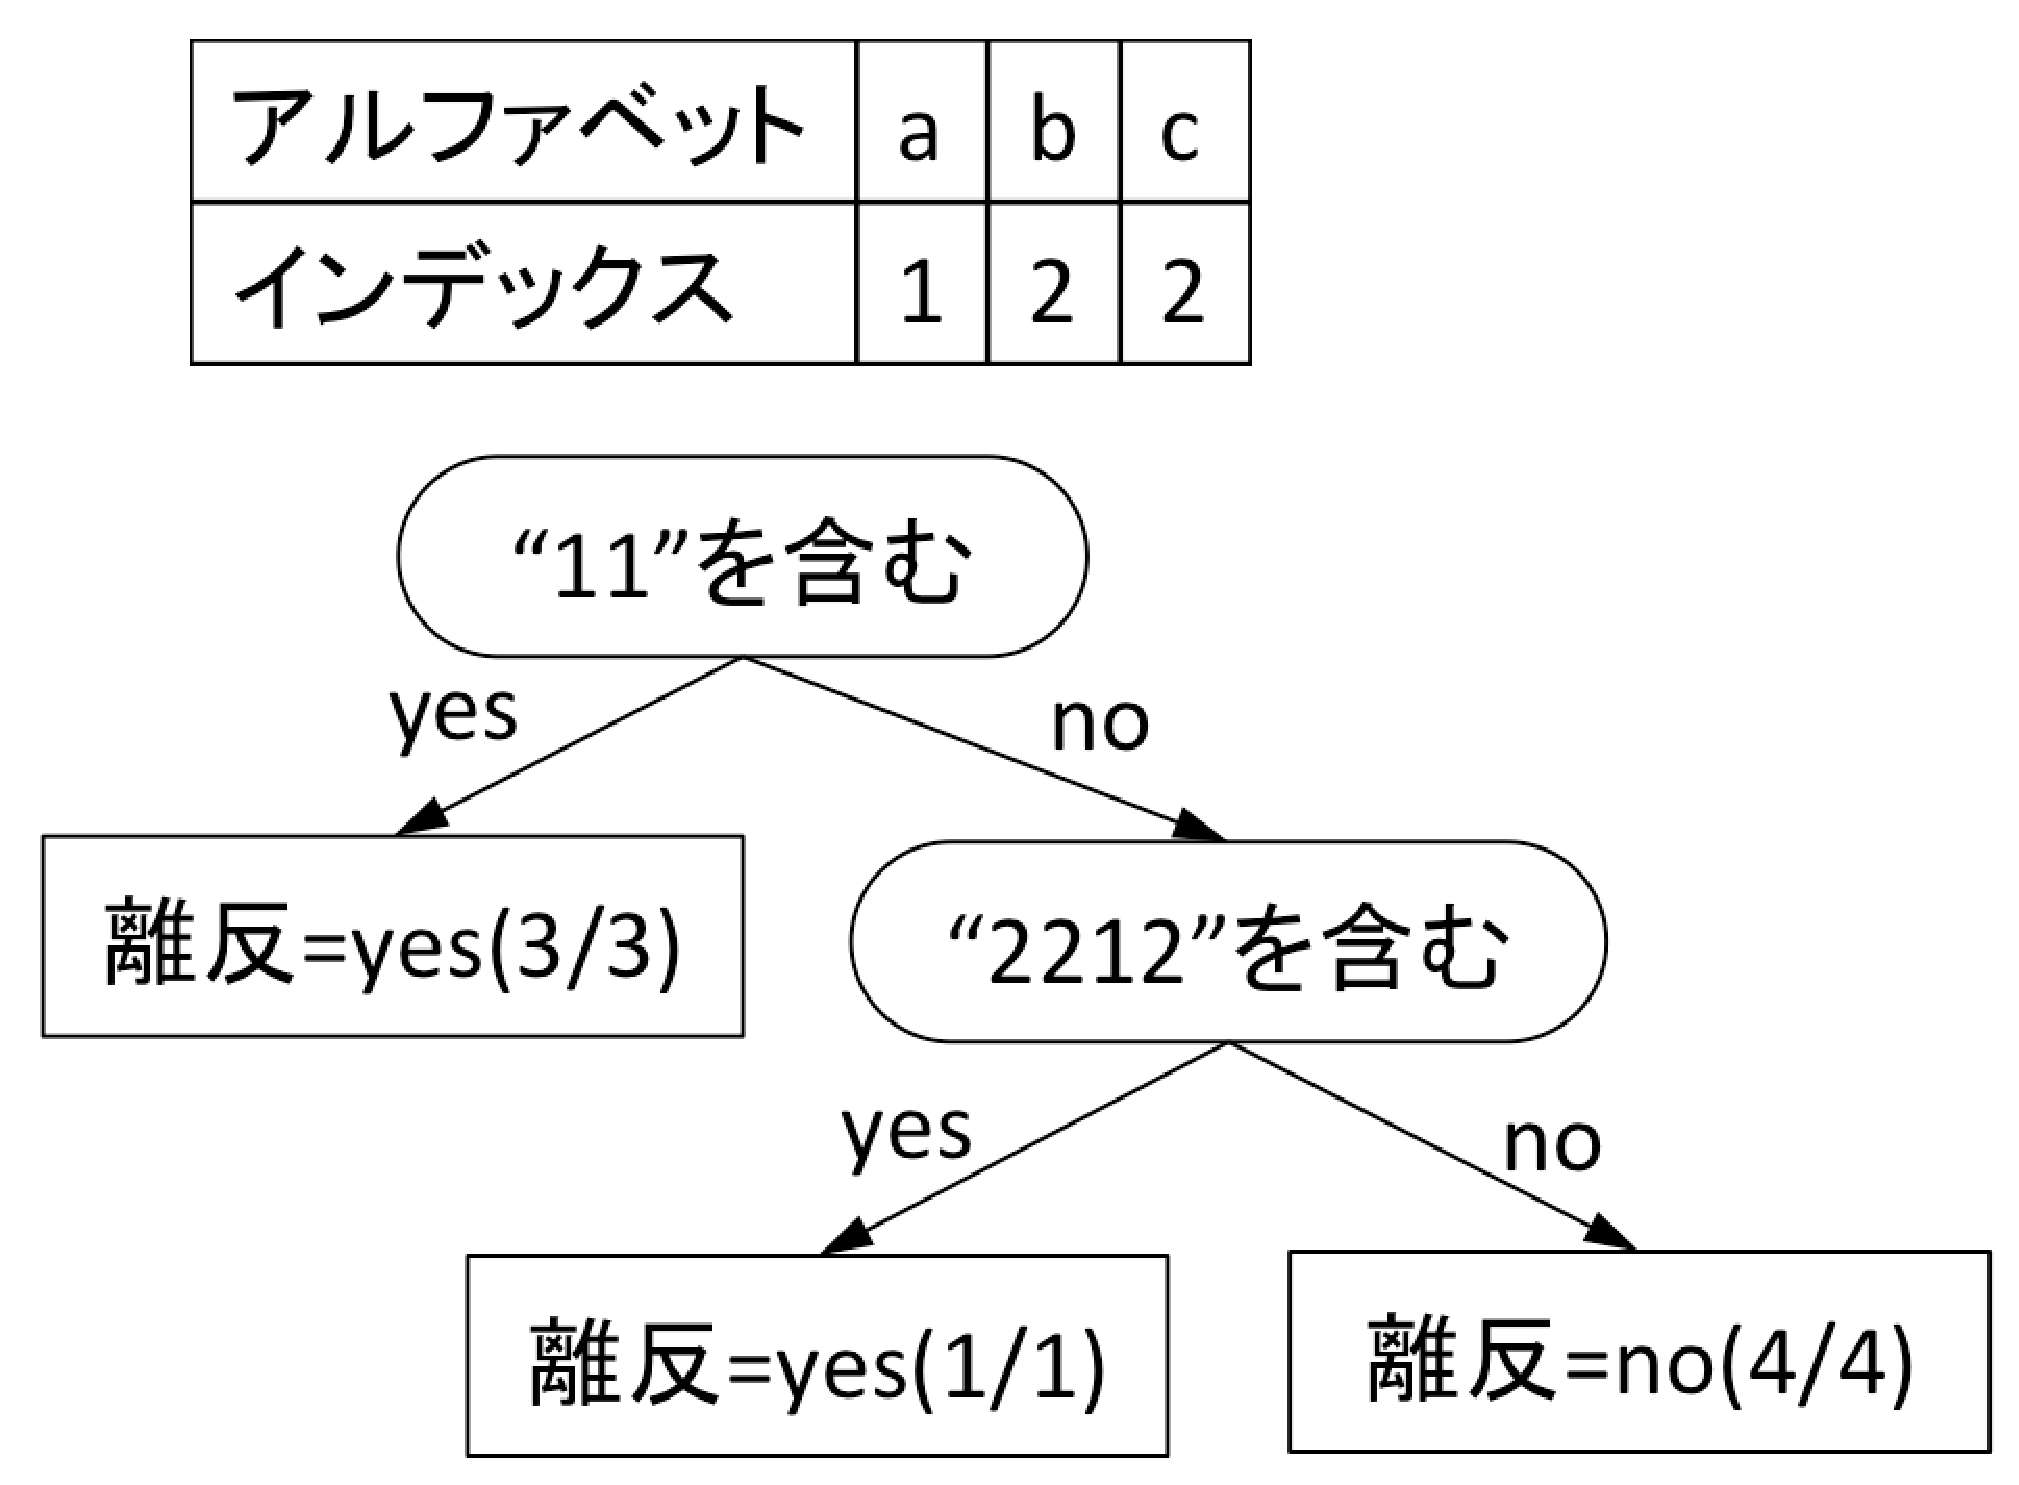
\includegraphics[scale=0.19,clip]{./figure/bonsai2.eps}
\caption{BONSAIによる離反顧客モデルの構築例}
\label{fig:mbonsai_bonsai2}
%\end{figure}
\end{center}
\end{minipage}

\end{tabular} 
\end{center}
\end{table} 

さらにBONSAIの特筆すべき特徴として、パターンを構成する要素(アルファベットと呼ぶ)を自動的にグルーピングする機能がある。
ここで、各アルファベットに対するグループをインデックスと呼ぶ。
例えば、\verb|a,b,c|の3つのブランドを2つのインデックスにグルーピングする仕方は3通りあるが((aとbc、bとac、cとab)、
それぞれのグルーピングに応じてオリジナルの系列のアルファベットを対応するインデックスで置換し、%(図ではaとbを1に、cを2に置換)、
上述の手順で決定木を3つ構築し、分類精度の最もよい決定木を選択する。
このようにして構築された決定木が図\ref{fig:mbonsai_bonsai2}に示されている。
%グルーピングをしない場合の決定木に比べて、よりシンプルな木が構成されていることが確認できる。
%また、
得られたグルーピングは、分類モデルの精度を高めるようなグルーピングになっているため、
そこから有用な知見が得られることが期待できる。
%上記の例であれば、ブランドaとbの連続購入が離反顧客に共通した特徴であり、それら2つのブランドは何らかの共通した特性を持っているのかもしれない。


\subsection{詳細}
以下では、決定木の構築に関する詳細について解説する。
\subsubsection{正規パターン}
アルファベット$\Sigma$上の$n$個の文字列定数を$\pi_1, \pi_2, ..., \pi_n$とし,
任意の$n+1$個の文字列を$x_0, x_1, ..., x_n$とした時,正規パターン(regular pattern,単に「系列パターン」とも呼ぶ)は,
$x_0\pi_1x_1\pi_2x_2 \cdots \pi_nx_n$の形式で与えられる.
データ検索の分野におけるワイルドカードを考えると理解しやすいであろう(ワイルドカードでは$x_i$の代わりに``*''が使われる).
本コマンドでは、上記の正規パターンの定義以外にも、$x_0\pi x_1$、
すなわち部分文字列$\pi$に限定した正規パターンも扱うことができる(以下、「文字列パターン」と呼ぶ)。
系列パターンと文字列パターンの切り替えは\verb|p=|の第2パラメータで指定する。

\subsubsection{先頭/末尾マッチ}
正規パターンの各サンプルの系列データへのマッチングルールとして、先頭一致と末尾一致を指定することができる。
それらの指定は\verb|p=|の第4(先頭一致),第5(末尾一致)パラメータで指定し、
文字数によって与える。この指定により、正規パターンの先頭(末尾)のアルファベットの位置が、
系列データの先頭(末尾)から指定の文字数以内であればマッチしたことになる。
例えば、系列データ\verb|aabccd|において、文字列パターン\verb|ab|は、先頭一致文字数が1であればマッチしないが、2であればマッチする。
\verb|ab|を系列パターンとすると、先頭一致文字列が1であってもマッチすることになる。
このパラメータを指定しなければ、以上のようなマッチングの制限はないものとして動作する。

\subsubsection{順序アルファベット}
順序構造のあるアルファベットを扱うことができる。
順序構造を仮定した場合、インデックスの生成規則に違いが出てくる。
アルファベット集合$\{a_1,a_2,\dots,a_n\}$について、
$a_1 \prec a_2 \prec \dots \prec a_n$の関係があるとすると、
連続する3つの任意のアルファベット$a_i,a_{i+1},a_{i+2}$について、
$\psi(a_i)=\psi(a_{i+2}) \Rightarrow \psi(a_i)=\psi(a_{i+1})$の関係が成り立つようにインデックスが生成される。
ここで、$\psi(a)$は、アルファベット$a$に対応させるインデックスを表す。
これは、あるグループに属するアルファベットは必ず連続するようにインデックス化されるということを意味する。
例えば、3つの順序アルファベット$a \prec b \prec c$について、$\{a,b\}と\{c\}$にグルーピングすることはあるが、
$\{a,c\}と\{b\}$にグルーピングすることはない。
順序アルファベットの指定は\verb|p=|の第3パラメータで指定する。

\subsubsection{最適なアルファベットインデックスの探索空間とローカルサーチ}
$n$個のアルファベットを$m$個以下のインデックスにグルーピングする場合の数は自明ではないが、
$m=2$に限れば、その数は$m^{n-1}$通り存在する。
$m,n$が共に小さい場合は、全ての場合について決定木を構築すればよいが、その値が大きい場合は以下に示すローカルサーチの手法によって部分空間を探索している。
それは、最初に各アルファベットに対応するインデックスをランダムに設定し、
その対応関係を少しずつ変更しながら決定木を構築し、分類精度に改善がなくなるまで変更を続けるというものである(
詳細は文献\cite{SSS94}を参照のこと)。
よって、アルファベットとインデックスの対応関係の初期値によって異なる結果が得られることもある。
そこで初期値を複数個用意して得られた結果から最適なモデルを選ぶ方法(マルチスタート)も用意されている。
本コマンドでは\verb|iter=|によって、初期値の個数を指定することが可能である。
デフォルトは\verb|iter=1|である。

\subsubsection{候補パターンの生成方法}
表\ref{tbl:mbonsai_inp2}に示されるような候補パターンは、ローカルサーチにおいてアルファベットインデックスが更新される度に新たに生成される。
決定木の節点における分類規則は、この候補パターンに基づいてなされるために、その生成方法は重要である。
本コマンドでは、以下に示すヒューリスティックな方法で候補パターンを列挙している。
まず、インデックスにおける長さ1の正規パターンを構築し、優先キューに格納する。
優先キューにおける優先順位は、正規パターンのエントロピー(後述)の昇順で決まる。
そして、優先キューからエントロピーの最も低い正規パターンを選択し、
その正規パターンにインデックスを一つ追加して、長さ2の正規パターンを構成し、再び優先キューに格納する。
上記の手順を繰り返し、途中、長さ$n$の正規パターンを選択すれば、長さ$n+1$の正規パターンが優先キューに格納される。
ただし、$n$が5を超えた場合はインデックスの追加は行わない(
正規パターンのサイズの上限の変更は\verb|p=|の第6パラメータで指定可能)。
そして、ユーザが指定した候補数(\verb|cand=|で指定)を超えれば終了する。
正規パターンの評価に用いるエントロピーは、決定木の節点における分岐ルールの選択にも用いられ、
正規パターンがクラスを極端な分布に分類すればするほど小さな値になる。
正規パターン$\pi$のエントロピー$ent(\pi)$は、式\ref{eq:mbonsai_entropy}で定義される。

\begin{equation}
ent(\pi)=-q^{{\rm m}(\pi)}\sum_{i=1}^c p_i^{{\rm m}(\pi)} \log p_i^{{\rm m}(\pi)}
            -q^{{\rm u}(\pi)}\sum_{i=1}^c p_i^{{\rm u}(\pi)} \log p_i^{{\rm u}(\pi)}
\label{eq:mbonsai_entropy}
\end{equation}

ここで、$c$はクラス数を表し、$p_i^{{\rm m}(\pi)}$($p_i^{{\rm u}(\pi)}$)は
正規パターン$\pi$がマッチした(しなかった)サンプルにおけるクラス$i$の構成比を表している
($\sum_i^c p_i^{{\rm m}(\pi)}=1$)。
また$q^{{\rm m}(\pi)}$($q^{{\rm u}(\pi)}$)は、正規パターン$\pi$がマッチした(しなかった)
サンプルの全サンプルに対する構成比である($q^{{\rm m}(\pi)}+q^{{\rm u}(\pi)}=1$)。

\subsubsection{その他の型の変数}
本コマンドでは、系列データ以外にも、数値とカテゴリ変数を説明変数として指定することができる。
そうすることで、正規パターンのルールと数値やカテゴリについてのルールが混在した決定木を構築することが可能となる。
数値やカテゴリの分岐規則に生成ついては、C4.5と同様の方法を利用している\cite{Quinlan93}。
本コマンドでは、\verb|p=,n=,d=|によって、系列項目、数値項目、カテゴリ項目の項目名をそれぞれ指定する。

\subsubsection{分岐ルールの選択}
本コマンドにおける決定木の構築は、2分岐によるトップダウンの貪欲法を採用している。
すなわち、木の節点における分割ルールは、その節点における情報のみに基づいた評価基準に従って決定される。
評価基準としては、
%式\ref{eq:mbonsai_entropy_gain}に示される
エントロピーゲインを最大にするような分岐ルールが選ばれる。
ある節点に分類されたサンプルについて、クラス$i$である確率(構成比)を$p_i$で表すと、
その節点におけるエントロピーは、$ent=-\sum_{i=1}^c p_i \log{p_i}$で計算される。
ここで、$p_i$は節点に分類されたサンプル数$n$とそのうちでクラス$i$に属するサンプル$n_i$との比$n_i/n$で計算される。
そして、式\ref{eq:mbonsai_entropy}で示された正規パターン$\pi$により分割した後のエントロピー$ent(\pi)$との差がエントロピーゲインである。
すなわち、これは正規パターン$\pi$によって分割することで、エントロピーをどの程度低減させるかを意味している。
このような分割を繰り返し、ある節点に分類される全てのサンプルが一つのクラスに属するか、
もしくはそれ以上分割できるなくなるまで木を成長させる。
このような決定木は最大木と呼ばれる。

\subsubsection{枝刈り}
前項で示した方法に従って最大木$T_{max}$を構築するが、
一般的に木のサイズが大きくなると、
モデルが訓練データに過適合(overfitting)することにより、
訓練データの分類精度は高まる(誤分類率が下がる)一方で、
未知データへの予測精度が下がってしまう。
この問題を回避するために、最大木よりサイズの小さな部分木(ただし根節点を含む)を選択する
「枝刈り(pruning)」を行う。

決定木$T$を節点$t$の集合として考え、最大木を$T_{max}=\{t_1,t_2,\dots,t_k\}$で、
そして節点$t$を根節点とした部分木を$T_t$で表すと、
節点$t\in P$を根節点とする部分木を全て枝刈りした(葉節点に置き換えた)決定木は
$T_{max}-\bigcup_{t\in P} T_t + P$で表される。
決定木$T$の誤分類率を$R(T)$で表すと、枝刈りとは、
未知データに対する誤分類率が最も低くなるような部分木$T^*$を選択する問題と考える事ができる。
$T$の未知データに対する真の誤分類率を直接求める事はできないので、
訓練データから推定することになる。
いま、その推定量を$C(T)$で表すと、
枝刈りは式\ref{eq:pruning}の通り定式化できる。

\begin{equation}
\argmin_{P\subseteq T_{max}} C(T_{max}-\bigcup_{t\in P} T_{t} + P)
\label{eq:pruning}
\end{equation}

この問題に対して、
本コマンドでは、コスト複雑性枝刈り(cost-complexity pruning)と呼ばれる方法\cite{Breiman84}を採用している。
この方法は、大きく二つのフェーズから構成さる。
まず訓練データを用いて構築された最大木からネストした一連の部分木
$T_1 \supset T_2 \supset \dots \supset T_k$を選択する
(ここで$T_1$は最大木、$T_k$は根節点のみからなる木と考えればよい)。
そして次に、それらの木の精度をテストサンプル法もしくは交差検証法(cross validation)によって推定し、
最も推定精度の高い木を選択する。

一連の部分木を選択するフェーズにおいては、
まず決定木$T$の評価関数としてコスト複雑性$R_{\alpha}(T)=R(T)+\alpha|\tilde{T}|$を定義し、
この値が小さい程良い木と考える。
この式は、決定木の誤分類率$R(T)$と決定木の複雑性$|\tilde{T}|$($T$の葉節点の数)のトレードオフを
複雑性パラメータ$\alpha(\ge 0)$によってバランスさせたものである。
訓練データにおいては、木のサイズが大きくなるに従い誤分類率$R(T)$は単調に減少するが、
逆に複雑性$|\tilde{T}|$は単調に増加する。
%また$\alpha(\ge 0)$はコスト複雑性パラメータと呼ばれ、モデルの誤分類率と複雑さを調整する役割を持つ。
そして$\alpha$を調整する事で、誤分類率と複雑性のどちらを優先するかが調整される。
ここで、$\alpha$を一つの値に固定すると、$R_{\alpha}(T)$を最小化しかつ最小サイズの部分木$T(\alpha)$が
ただ一つ存在することが知られている。
さらに、$\alpha$を小さい区間を単位として変化させていったとき、それぞれの$\alpha$に対応する$T(\alpha)$
を列挙でき、結果として、ネストした部分木列$T_1 \supset T_2 \supset \dots \supset T_k$が構築される
(より詳細は\cite{Breiman84}を参照のこと)。
ここで、部分木$T_i$は$\alpha \in (\alpha_i,\alpha_{i+1}]$においてコスト複雑性最小かつ最小サイズの決定木である。
以上により、ネストした一連の部分木と、それぞれの木に対応するコスト複雑性パラメータ$\alpha_1,\alpha_2,\dots,\alpha_k$が得られる。

そして次に、以上の方法により得られた一連の部分木の中から、
未知データに対する推定誤分類率を最も低めるような最適な部分木$\hat{T}^*$を選択する。
本コマンドでは、誤分類率の推定にテストサンプル法(\verb|ts=|を指定)もしくは交差検証法(\verb|cv=|を指定)を選ぶことができる。
テストサンプル法では、訓練データ$D$を$1:2$の割合で$D_1,D_2$に分割する。
そして、$D_2$を訓練データとして最大木を構築し、前フェーズで得た複雑性パラメータ$\alpha_1,\alpha_2,\dots,\alpha_k$それぞれに対応する
部分木を選択し、その部分木によって$D_1$を未知データとして予測した結果を未知データの誤分類率の推定値とする。
交差検証法においては、訓練データ$D$を均等に$n$分割し、$D_1,D_2,\dots,D_n$を得る。
最初に$D_1$を未知データとして、そしてその他を訓練データとしてテストサンプル法と同様の推定を行う。
同様に残りの$D_2$〜$D_n$をそれぞれテストデータとして、同様のプロセスを$n$回実施することで、
全ての訓練データ$D$を一回ずつ未知データとして検証する事になる。
そのようにして得られた平均誤分類率を未知データの推定値とする。
上記の結果得られた一連の複雑性パラメータ$\alpha_1,\alpha_2,\dots,\alpha_k$に対応する決定木
$T_1, T_2, \dots, T_k$
のうち、誤分類率が最も低い決定木を最適な決定木として選択する。
また、最小誤分類率に標準誤差を加えた誤分類率より小さい部分木の中から、
サイズの最も小さいサイズの木を選ぶ事も可能である(これは「1SEルール」と呼ばれる)。

なお、テストサンプル法もしくは交差検証法を用いず、$\alpha$の値を直接指定する事で枝刈りを実現する事もできる。
この方法は、推定のための計算が不要なために決定木を高速に構築できるが、一方で$\alpha$の値の指定が恣意的になるという欠点がある。

%本コマンドで採用している枝刈りは、C4.5で採用されている枝刈りと同様の方法で、誤分類削減枝刈り(reduced error pruning)と呼ばれる\cite{Quinlan93}。
%この方法では、統計的推定の考え方を取り入れ,枝刈りをする前後での誤分類率の推定値の大小によって、枝刈りをすべきかどうかを判定する。
%推定値として、観測された誤分類率から信頼区間の上限値を誤分類率の推定値として利用する。
%いま,ある葉節点に$n$件の訓練データが分類され,そのうち$e$件が誤分類であったとする.
%ここで次のような仮定を置く.すなわち,真の誤分類率$\epsilon$のもと,$n$回の試行で$e$回の誤分類を観測したというベルヌーイ試行を仮定する.
%そうすると,誤分類数$e$は二項分布$B(n,\epsilon)$ に従う確率変数となる.
%信頼係数$1-\alpha$における,真の誤分類率の推定区間の上限値は式
%(\ref{math:esterr})を満たす$\epsilon$となる.

%\begin{equation}
%\sum_{x=0}^{e} {n \choose x} \epsilon^x (1-\epsilon)^{n-x}=\alpha/2
%\label{math:esterr}
%\end{equation}

%以上のようにして求めた推定誤分類率を用いて,葉節点のみを子節点として持つ親節点について,
%子節点の推定誤差率の合計と親節点の推定誤差率とを比較して,
%親節点の推定誤差率の方が小さければ,子節点は枝刈りされ,親節点を葉節点に置換する.
%以上の手順を順次適用し,刈るべき枝がなくなるまで繰り返す.
%本コマンドでは$\alpha$を\verb|prune=|パラメータで指定することによって枝刈りのレベルを調整する。
%$\alpha$のデフォルトは0.25、すなわち信頼係数0.75である。
%$\alpha=1.0$とした場合(\verb|prune=100|)、
%サンプル数に大小に関わらず信頼区間の上限は点推定の値となるため、
%枝刈りは全く行われず、最大木が出力される(たとえサンプル1件であっても分割したほうが推定誤分類率は下がる)。
%逆に$\alpha$の値を0に近づけるほど、多くの枝が刈られることになる。

\subsubsection{枝刈りの実際}
本コマンドの枝刈りは、モデル構築モードにおいて、\verb|ts=|、\verb|cv=|、\verb|alpha=|のいずれかのパラメータを指定する事で実施される。
\verb|ts=|もしくは\verb|cv=|が指定された時は、テストデータを使った推定により、誤分類率最小のモデルが選択される。
また、\verb|alpha=|を指定した時は、指定の$\alpha$に応じた枝刈りのモデルが選択される。
\verb|model.txt|と\verb|model_info.txt|に出力される決定木やモデル評価は、選択されたモデルに基づいている。
ただし、いずれの指定においても、内部では最大木と全ての$\alpha$に対する枝刈りを計算しており、
予測モード(\verb|-predict|)において、再度\verb|alpha=|を指定することで、異なるモデルを用いた予測も可能となる。

\subsubsection{コスト考慮学習}
分類モデルの応用においては、分類精度(正答率)を高めるのではなく、
誤分類によって生じるコスト(誤分類コスト)を低減させる方が有用なケースが多くある。
離反顧客を離反しない顧客と予測した場合のコストと、
離反しない顧客を離反すると予測した場合のコストは、それぞれで実施する施策を考慮するとそのコストは異なるかもしれない。
このようなコストを考慮に入れてモデルを構築することを、一般的にコスト考慮学習(cost sensitive learning)と呼ぶ。
その方法は多数提案されているが、ここでは、Breimanらの提案する方法を用いている\cite{Breiman84}。
この方法は、分岐ルールの計算において、サンプルがクラス$i$である確率$p_i$の計算をコストによる加重により修正するというものである。
いま、クラス$j$をクラス$i$と予測したときのコストを$c(i|j)$で表すと、クラス$i$のコスト合計$\sum_{j}c(i|j)$を
クラス$i$の加重として確率$p_i$を修正する。
コスト計が大きいクラス$i$は、常にサンプル数が水増しされることになり(オーバーサンプリング)、
クラス$i$の情報に敏感なモデルが構築されることになる。
クラスファイルは表\ref{tbl:mbonsai_cost}に示されるように、
実クラス(\verb|real|)に対する予測クラス(\verb|predict|)のコスト(\verb|cost|)を一行とするCSVファイルで指定する。
実クラスと予測クラスの特定の組み合わせを省略した場合、
もしくはコストファイルそのものを省略した場合、
実クラスと予測クラスが同じ場合のコストは0、異なる場合は1と設定される。

\begin{table}[htbp]
\begin{center}
\begin{tabular}{c}

\begin{minipage}{0.7\hsize}
\begin{center}
\caption{離反モデルにおけるコストの指定例。
1行目は、離反クラスがyesのサンプルをnoと予測した場合のコストが2で、
2行目は、離反クラスがnoのサンプルをyesと予測した場合のコストが5と設定されている。
項目名は任意であるが、順序は、実クラス、予測クラス、コストの順番でなければならない。
\label{tbl:mbonsai_cost}}
{\small
\begin{tabular}{llc}
\hline
real&predict&cost \\
\hline
yes & no  & 2 \\
no  & yes & 5 \\
\hline
\end{tabular} 
}
\end{center}
\end{minipage}

\end{tabular} 
\end{center}
\end{table} 





\subsection{出力データ}
本コマンドで出力される各種データファイルが表\ref{tbl:mbonsai_out}にまとめられている。

\begin{table}[htbp]
\begin{center}
\begin{tabular}{ll}

\begin{minipage}{1.0\hsize}
\begin{center}
\caption{本コマンドがモデル構築モードで出力するデータ一覧\label{tbl:mbonsai_out}}
{\small
\begin{tabular}{lll}
\hline
ファイル名&内容&備考\\
\hline
\verb|model.pmml|       & PMML\footnote{
Predictive Model Mark-up Languageの略で、
数理モデルをXMLにより表現する業界標準である。
PMMLに準拠はしているが、本コマンド特有の拡張タグも利用していることに留意されたい。
}
による決定木モデル                                                   & 枝刈り情報を伴った最大木が出力されている。\\
                          &                                          & \verb|-predict|指定時の予測モードで利用される。 \\
\verb|alpha_list.csv|     & 複雑度パラメータ$\alpha$別のモデル情報   & 一連の$\alpha$に応じたモデルの精度やサイズなど。 \\
\verb|model_min.txt|      & 推定誤分類率最小の枝刈りモデルの要約     & \verb|cv=| もしくは \verb|ts=|を指定したときのみ出力される。 \\
\verb|model_1se.txt|      & 同じく1SEルールの枝刈りモデルの要約      & \verb|cv=| もしくは \verb|ts=|を指定したときのみ出力される。 \\
\verb|model.txt|          & 指定の$\alpha$による枝刈りモデルの要約   & \\
\verb|model_info_min.csv| & 推定誤分類率最小の枝刈りモデルの各種情報 & \verb|cv=| もしくは \verb|ts=|を指定したときのみ出力される。  \\
\verb|model_info_1se.csv| & 同じく1SEルールの枝刈りモデルの各種情報  & \verb|cv=| もしくは \verb|ts=|を指定したときのみ出力される。  \\
\verb|model_info.csv|     & 指定の$\alpha$による枝刈りモデルの要約   & \\
\verb|predict_min.csv|    & 推定誤分類率最小の枝刈りモデルによる予測 & \verb|cv=| もしくは \verb|ts=|を指定したときのみ出力される。  \\
\verb|predict_1se.csv|    & 同じく1SEルールの枝刈りモデルによる予測  & \verb|cv=| もしくは \verb|ts=|を指定したときのみ出力される。  \\
\verb|predict.csv|        & 指定の$\alpha$による枝刈りモデルによる予測 & \\
\verb|param.csv|          & 実行パラメータ一覧                       & パラメータのキーワードと値のペアを出力 \\
\hline
\end{tabular} 
}
\end{center}
\end{minipage}

\end{tabular} 
\end{center}
\end{table} 

\paragraph{model.pmml}
ここで出力される決定木は最大木で、
各節点には以下に示されるように\verb|complexity penalty|属性が示されており、
$\alpha$がその値より大きい場合に、その枝は刈られる事になる。
PMMLにモデルとしての最大木と枝刈り情報を記録しているので、
予測モードでの実行時に$\alpha$を指定することで、その値に応じた決定木モデルにより予測することが可能となる。
\begin{Verbatim}[baselinestretch=0.7,frame=single]
              :
<Node id="0" score="yes" recordCount="8" >
    <Extension extender="KGMOD" name="complexity penalty" value="0.500000"/>
              :
\end{Verbatim}

\paragraph{model\_min.txt,model\_1se.txt,model.txt}
PMMLデータと異なり、枝刈り後のモデルの要約がテキスト形式で出力される。
\verb|[alphabet-index]|の欄には、アルファベットとインデックスの対応関係が示されている。
以下の例では、アルファベット\verb|c|がインデックス\verb|1|に、\verb|b,a|がインデックス\verb|2|に対応している。
決定木に表示されるパターンの分岐規則はこのインデックス記号によって示される。
\begin{Verbatim}[baselinestretch=0.7,frame=single]
[alphabet-index]
Field Name: ブランド系列
Index[1]={c}
Index[2]={b,a}
\end{Verbatim}
\verb|[decision tree]|の欄には、決定木がテキスト形式で示され、その下にはモデルサイズ(葉節点の数)と最も深い葉の階層数が示される。
\begin{Verbatim}[baselinestretch=0.7,frame=single]
[decision tree]
if($ブランド系列 has 22)
  then $離反=yes (hit/sup)=(4/4)
  else $離反=no (hit/sup)=(4/4)

number of leaves: 2
deepest level: 1
\end{Verbatim}

\verb|[Confusion Matrix by Training]|の欄には、
訓練データを決定木モデルで予測した場合の分類結果が示されている。
また、コストによる分類表、クラス別の予測精度、全体の予測精度も示されている。
\verb|[Confusion Matrix by Estimation]|の欄は、\verb|ts=|もしくは\verb|cv=|を指定した時のみ出力される。
内容は\verb|[Confusion Matrix by Training]|の欄と同様であるが、テストデータによる結果であることが異なる点である。

\begin{Verbatim}[baselinestretch=0.7,frame=single]
[Confusion Matrix]
## TRAINING DATA ##
## By count
         Predicted As ...
        yes     no      Total
yes     4       0       4
no      0       4       4
Total   4       4       8

## By cost
         Predicted As ...
        yes     no      Total
yes     0       0       0
no      0       0       0
Total   0       0       0

## Detailed accuracy by class
class,recall,precision,FPrate,F-measure
yes,1,1,0,1
no,1,1,0,1

## Summary
accuracy=1
totalCost=0
\end{Verbatim}

最後に\verb|[Selected Alpha]|の欄には、枝刈りにおいて採用された複雑度パラメータの値が出力されている。
\begin{Verbatim}[baselinestretch=0.7,frame=single]
[Selected Alpha]
alpha: 0
\end{Verbatim}


\paragraph{predict\_min.txt,predict\_1se.txt,predict.txt}
モデル構築に用いた訓練データに決定木モデルによる予測結果を追加したCSVデータである。
予測結果は、以下に示すように、\verb|predict|項目に予測確率の最も高かったクラス名が出力され、
さらに各クラス毎(以下では\verb|yes|と\verb|no|)に予測確率が出力される。
\verb|ts=|が指定された場合は、テストデータの予測結果が出力され、
\verb|cv=|が指定された場合は、交差検証における全テストデータの予測結果が出力される。
また、\verb|alpha=|が指定された場合は、訓練データそのものの予測結果が出力される。

\begin{Verbatim}[baselinestretch=0.7,frame=single]
ブランド系列,離反,predict,yes,no
bcaba,yes,yes,1,0
bcabcaa,yes,yes,1,0
aaabac,yes,yes,1,0
caa,yes,yes,1,0
cca,no,no,0,1
cacbc,no,no,0,1
bcc,no,no,0,1
acca,no,no,0,1
\end{Verbatim}

\paragraph{model\_info\_min.csv,model\_info\_1se.csv,model\_info.csv}
これらのファイルは、モデル情報をCSV形式で出力したものである。
\verb|nobs|は訓練データの件数、\verb|alpha=|は枝刈りの複雑度パラメータの値、
\verb|accuracy,totalCost|はテストデータにおけるモデルの正答率と総コストである。
\begin{Verbatim}[baselinestretch=0.7,frame=single]
nobs,alpha,accuracy,totalCost
8,0,1,0
\end{Verbatim}

\paragraph{alpha\_list.csv}
枝刈りの複雑度パラメータ$\alpha$の値別に、それぞれに対応する枝刈りされた決定木の
エラー率、標準誤差、エラー率±標準誤差の値が示されている。
\begin{Verbatim}[baselinestretch=0.7,frame=single]
alpha    ,leafSize,errorRate,SE     ,up     ,lo
0        ,102     ,0.0082   ,0.0015 ,0.0098 ,0.0066
8.15e-05 , 98     ,0.0085   ,0.0016 ,0.0101 ,0.0069
9.41e-05 , 91     ,0.0091   ,0.0016 ,0.0108 ,0.0074
0.000124 , 82     ,0.0100   ,0.0017 ,0.0118 ,0.0083
    :       :         :         :       :       : 
0.035669 ,  2     ,0.0878   ,0.0049 ,0.0927 ,0.0828
1.79e+308,  1     ,0.1399   ,0.0060 ,0.1460 ,0.1339
\end{Verbatim}

\paragraph{param.csv}
モデル構築時に用いられた各種パラメータの値がCSV形式により格納されている。

\newpage
\subsection{書式1:モデル構築モード}
\begin{verbatim}
mbonsai i= [p=] [n=] [d=] c= O= [delim=] [cost=] [seed=] [cand=] [iter=] [cv=|ts=]
        [leafSize=] [--help]
\end{verbatim}

\begin{table}[htbp]
{\small
\begin{tabular}{ll}

\verb|i=|     & : 訓練データファイル名 \\
\verb|p=|     & : パターン項目名(複数指定可) \\
              & : 項目名の後にコロンで区切って5つのパラメータを指定できる。 \\
              & : \verb|p=項目名:is:seq:ordered:head:tail:rs| \\
              & : \verb|is|: インデックスのサイズ \\
              & : \ \  指定を省略すれば、インデックスを生成せず、オリジナルのアルファベットのパターンを用いる。 \\
              & : \verb|seq|: パターンの種類 \\
              & : \ \ true:部分系列パターン \\
              & : \ \ false:部分文字列パターン(default) \\
              & : \verb|ordered|: インデックスの生成において、アルファベットに順序があると仮定するかどうか。 \\
              & : \ \ \ \ (\verb|is|の指定を省略していれば無視される) \\
              & : \ \ true: 順序あり, アルファベットをある閾値以上/未満でグルーピングする。 \\
              & : \ \ false: 順序なし(default) \\
              & : \verb|head|: 先頭一致の先頭からの文字数(デフォルトは先頭一致を考慮しない) \\
              & : \verb|tail|: 末尾一致の先頭からの文字数(デフォルトは末尾一致を考慮しない) \\
              & : \verb|rs|: 正規パターンのサイズ上限(デフォルトは5) \\
\verb|n=|     & : 数値項目名(複数指定可) \\
\verb|d=|     & : カテゴリ項目名(複数指定可) \\
\verb|c=|     & : クラス項目名 \\
\verb|O=|     & : 出力ディレクトリ名(text,PMMLによるモデル,モデル統計など) \\
\verb|delim=| & : パターンの区切り文字(デフォルト:空文字,すなわち1バイト文字を1つのアルファベットと見なす) \\
\verb|cost=|  & : コストファイル名 \\
\verb|seed=|  & : 乱数の種(default=-1:時間依存) \\
\verb|cand=|  & : 説明変数としてのパターン数(default=30,範囲:1〜256) \\
\verb|iter=|  & : ローカルサーチ回数(default=1) \\
%\verb|prune=| & : 枝刈り度(default=25,範囲:0〜100,この値が小さければ木のサイズは小さくなる) \\
%\verb|treeSize=| & : 決定木のサイズ上限(決定木のサイズはリーフ数で指定する,default:制限なし) \\
%                 & : 枝刈りの過程で生成される一連の$\alpha_i$について、対応する決定木$T_i$のリーフ数が、\\
%                 & : ここで指定した値より大きければ、そのような$\alpha_i$および$T_i$は、出力の対象としない。\\
\verb|leafSize=| & : 一つのリーフに含まれるサンプル数の下限(default:制限なし) \\
\verb|alpha=|    & : 枝刈り度を指定する。省略時は0.01が設定される。ただし、\verb|ts=|もしくは\verb|cv=|を指定した場合、\\
                 & : このパラメータは無効化される。\\
\verb|ts=|       & : テストサンプル法によるテストデータの割合を指定する。値を省略して"\verb|ts=|"と指定すると0.333が用いられる。 \\
\verb|cv=|       & : 交差検証法によるデータの分割数を指定する。値を省略して"\verb|cv=|"と指定すると10が用いられる。 \\
                 & : \verb|ts=,cv=|のいずれも指定されていない場合は、\verb|alpha=0.01|と指定されたと見なされる。\\
                 & : \verb|alpha=,ts=,cv=|を指定したとしても、PMMLに最大木と枝刈り度が記録されるので、\\
                 & : 予測モードにおいて、\verb|alpha|の値を変更して予測することが可能である。\\
%\verb|-1se|      & : 枝刈りにおいて、1SE(標準誤差)基準を用いる。\\
\verb|--help|    & : ヘルプの表示 \\

\end{tabular} 
}
\end{table} 

\newpage
\subsection{書式2:予測モード}

\begin{verbatim}
       mbonsai -predict i= I= o= [alpha=] [--help]
\end{verbatim}

\begin{table}[htbp]
{\small
\begin{tabular}{ll}
\verb|-predict| & : 予測モードで動作させる。予測モードでは必須 \\
\verb|i=|       & : 入力データ【必須】 \\
                & : 項目名は、モデル構築モードで利用した項目と同じでなければならない。 \\
\verb|I=|       & : モデル構築モードでの出力先ディレクトリパス【必須】 \\
                & : 利用するファイルは以下のとおり。 \\
                & :   bonsai.pmml: pmmlによる決定木モデル  \\
\verb|o=|       & : 予測結果ファイル名 \\
                & :   入力データに"predict"という項目を追加して出力する。\\
                & : 項目名は、モデル構築モードで利用した項目と同じでなければならない。 \\
\verb|alpha=|   & : 枝刈りの複雑度パラメータ。 \\
                & : 0以上の実数値を与える以外に、以下の2つは特殊な意味を持つシンボルとして指定できる。 \\
                & :   min: 推定誤分類率最小の枝刈りモデルに対応する$\alpha$の値。\\
                & :   1se: 同じく1SEルールの枝刈りモデルに対応する$\alpha$の値。\\
                & :        これら2つのシンボルによる指定は、モデル構築時に\verb|ts=|もしくは\verb|cv=|を指定した時のみ有効である。\\
                & : 省略時の動作:\\
                & : モデル構築時に\verb|ts=|もしくは\verb|cv=|を指定した場合は、\verb|min|が用いられる。\\
                & : モデル構築時に\verb|alpha=|を指定した場合は、その値が用いられる。 \\
\verb|delim=|   & : パターンの区切り文字(デフォルト:空文字,すなわち1バイト文字を1つのアルファベットと見なす) \\
\verb|--help|   & : ヘルプの表示\\

\end{tabular} 
}
\end{table} 


\subsection{利用例}
\subsubsection{例1 モデル構築の例}
ここでは、\verb|ts=,cv=,alpha=|のいずれも指定されていないので、\verb|alpha=0.01|で枝刈りされた結果が\verb|model.txt|に出力される。
\begin{Verbatim}[baselinestretch=0.7,frame=single]
$ more input.csv
ブランド系列,離反
bcaba,yes
bcabcaa,yes
aaabac,yes
caa,yes
cca,no
cacbc,no
bcc,no
acca,no

$ mbonsai p=ブランド系列:2 c=離反 i=input.csv O=result1

$ more result1/model.txt

[alphabet-index]
Field Name: ブランド系列
Index[1]={a}
Index[2]={b,c}

[decision tree]
if($ブランド系列 has 11)
  then $離反=yes (hit/sup)=(3/3)
  else if($ブランド系列 has 2212)
    then $離反=yes (hit/sup)=(1/1)
    else $離反=no (hit/sup)=(4/4)

numberOfLeaves=3
deepestLevel&=& 2

[Confusion Matrix by Training]
## By count
         Predicted As \ldots
	yes	no	Total
yes	4	0	4
no	0	4	4
Total	4	4	8

## By cost
         Predicted As \ldots
	yes	no	Total
yes	0	0	0
no	0	0	0
Total	0	0	0

## Detailed accuracy by class
class,recall,precision,FPrate,F-measure
yes,1,1,0,1
no,1,1,0,1

## Summary
accuracy=1
totalCost=0

$ more result1/model.pmml
<?xml version="1.0" encoding="UTF-8"?>
<PMML version="4.0">
  <Header copyright="KGMOD">
    <Application name="mclassify" version="1.0"/>
    <Timestamp>2014/07/20 23:00:13</Timestamp>
  </Header>
  <DataDictionary numberOfFields="2">
    <DataField name="ブランド系列" optype="categorical" dataType="string">
      <Value value="b"/>
      <Value value="c"/>
      <Value value="a"/>
    </DataField>
    <DataField name="離反" optype="categorical" dataType="string">
      <Value value="yes"/>
      <Value value="no"/>
    </DataField>
  </DataDictionary>
  <TreeModel functionName="classification" splitCharacteristic="binarySplit">
    <MiningSchema>
      <MiningField name="ブランド系列">
        <Extension extender="KGMOD" name="alphabetIndex">
          <alphabetIndex alphabet="b" index="2"/>
          <alphabetIndex alphabet="c" index="1"/>
          <alphabetIndex alphabet="a" index="2"/>
        </Extension>
      </MiningField>
      <MiningField name="離反" usageType="predicted"/>
    </MiningSchema>
    <Node id="0" score="yes" recordCount="8">
      <Extension extender="KGMOD" name="pruning" value="0.000000"/>
      <True/>
      <ScoreDistribution value="yes" recordCount="4"/>
      <ScoreDistribution value="no" recordCount="4"/>
      <Node id="1" score="yes" recordCount="4">
        <Extension extender="KGMOD" name="pruning" value="0.000000"/>
        <Extension extender="KGMOD" name="patternPredicate" value="substring">
          <SimplePredicate field="ブランド系列" operator="contain">
            <index seqNo="1" value="2"/>
            <index seqNo="2" value="2"/>
          </SimplePredicate>
        </Extension>
        <ScoreDistribution value="yes" recordCount="4"/>
        <ScoreDistribution value="no" recordCount="0"/>
      </Node>
      <Node id="2" score="no" recordCount="4">
        <Extension extender="KGMOD" name="pruning" value="0.000000"/>
        <Extension extender="KGMOD" name="patternPredicate" value="substring">
          <SimplePredicate field="ブランド系列" operator="notcontain">
            <index seqNo="1" value="1"/>
            <index seqNo="2" value="1"/>
          </SimplePredicate>
        </Extension>
        <ScoreDistribution value="yes" recordCount="0"/>
        <ScoreDistribution value="no" recordCount="4"/>
      </Node>
    </Node>
  </TreeModel>
</PMML>
\end{Verbatim}

\subsubsection{例2 例1のモデルから未知データを予測する}
構築した決定木モデルで未知データ(以下では訓練データを未知データとして使っている)を予測する例。
予測結果としては、各クラスの予測確率(\verb|yes,no|項目)、
およびその確率が最も高いクラス名(\verb|predict|項目)が出力される。
\begin{Verbatim}[baselinestretch=0.7,frame=single]
$ more unknown.csv
ブランド系列
bcaba
bcabcaa
aaabac
caa
cca
cacbc
bcc
acca

$ mbonsai -predict i=unknown.csv I=result1 o=predict.csv

$ more predict.csv
ブランド系列,predict,yes,no
bcaba,yes,1,0
bcabcaa,yes,1,0
aaabac,yes,1,0
caa,yes,1,0
cca,no,0,1
cacbc,no,0,1
bcc,no,0,1
acca,no,0,1
\end{Verbatim}

